\section{Error handling}
It is very important that a programmer knows if the code he is writing is correct or not, so it's very important that the compiler tells him of any errors it encounters. 
Our compiler can catch errors after every parsing of the code it does, and it will also complete the parse, so it can report every error encountered in that parse. \newline
To make the compiler easier to use, we have tried to make the error messages very descriptive. 
The programmer also gets a choice of whether he wants to print the compilation, and error markers will be printed in the correct places if he does.
We have also made it so the programmer can recompile his code once he has corrected any errors without restarting the compiler.

\begin{figure}[H]
\begin{center}
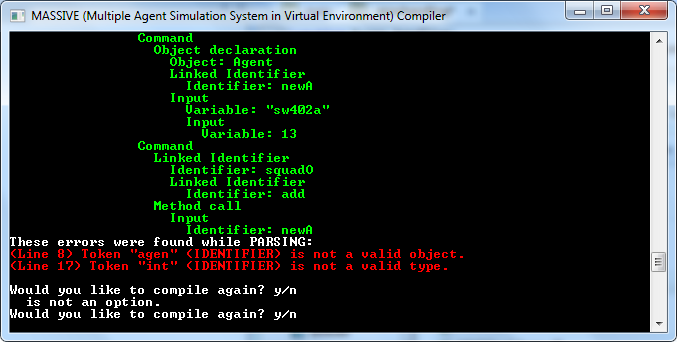
\includegraphics[scale=0.9]{Images/errorhandling.png}
\end{center}
\caption{An example of how the compiler handles errors.}
\end{figure}